While the analysis may be correct, it is not particularly convincing unless one is familiar with the probability theory. This is
where the simulation is helpful. By generating $1000$ samples of sizes from $n=1$ to $n=1000$, we can calculate the proportion of
samples for which the estimator was ``within $\ep$'' of the true parameter. By then plotting this proportion against sample size
we should see convergence for $\tilde{\lambda}_1$ but no convergence for $\tilde{\lambda}_2$. Note that I chose a small value of
$\lambda$ for my true parameter so that it converged more quickly and my laptop could finish the simulation. Indeed as $n$ gets
larger, the proportion of $\tilde{\lambda}_1$ that is ``within $\ep$'' of $\lambda$ is close to $1$. But the proportion of
$\tilde{\lambda}_2$ that is ``within $\ep$'' of $\lambda$ does not converge to anything.

\begin{center}
	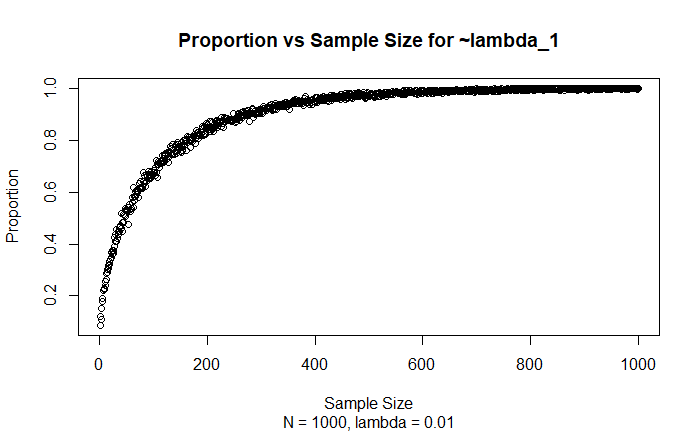
\includegraphics[scale=0.8]{proportion_plot_lambda_1.png}
	
	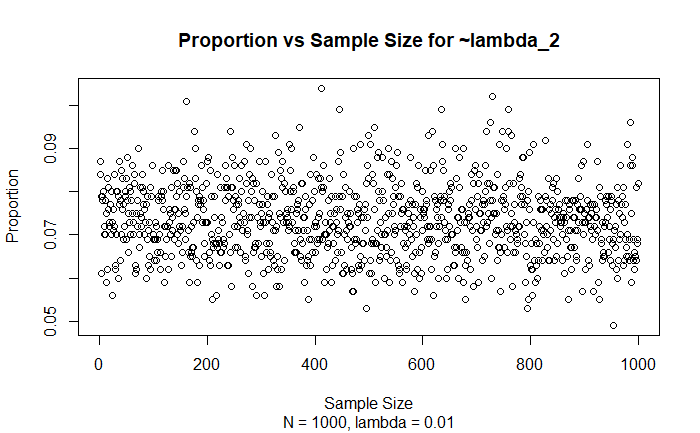
\includegraphics[scale=0.8]{proportion_plot_lambda_2.png}
\end{center}
